\section{YARN-Modell}\label{sec:yarnModel}

\begin{figure}
	\centering
	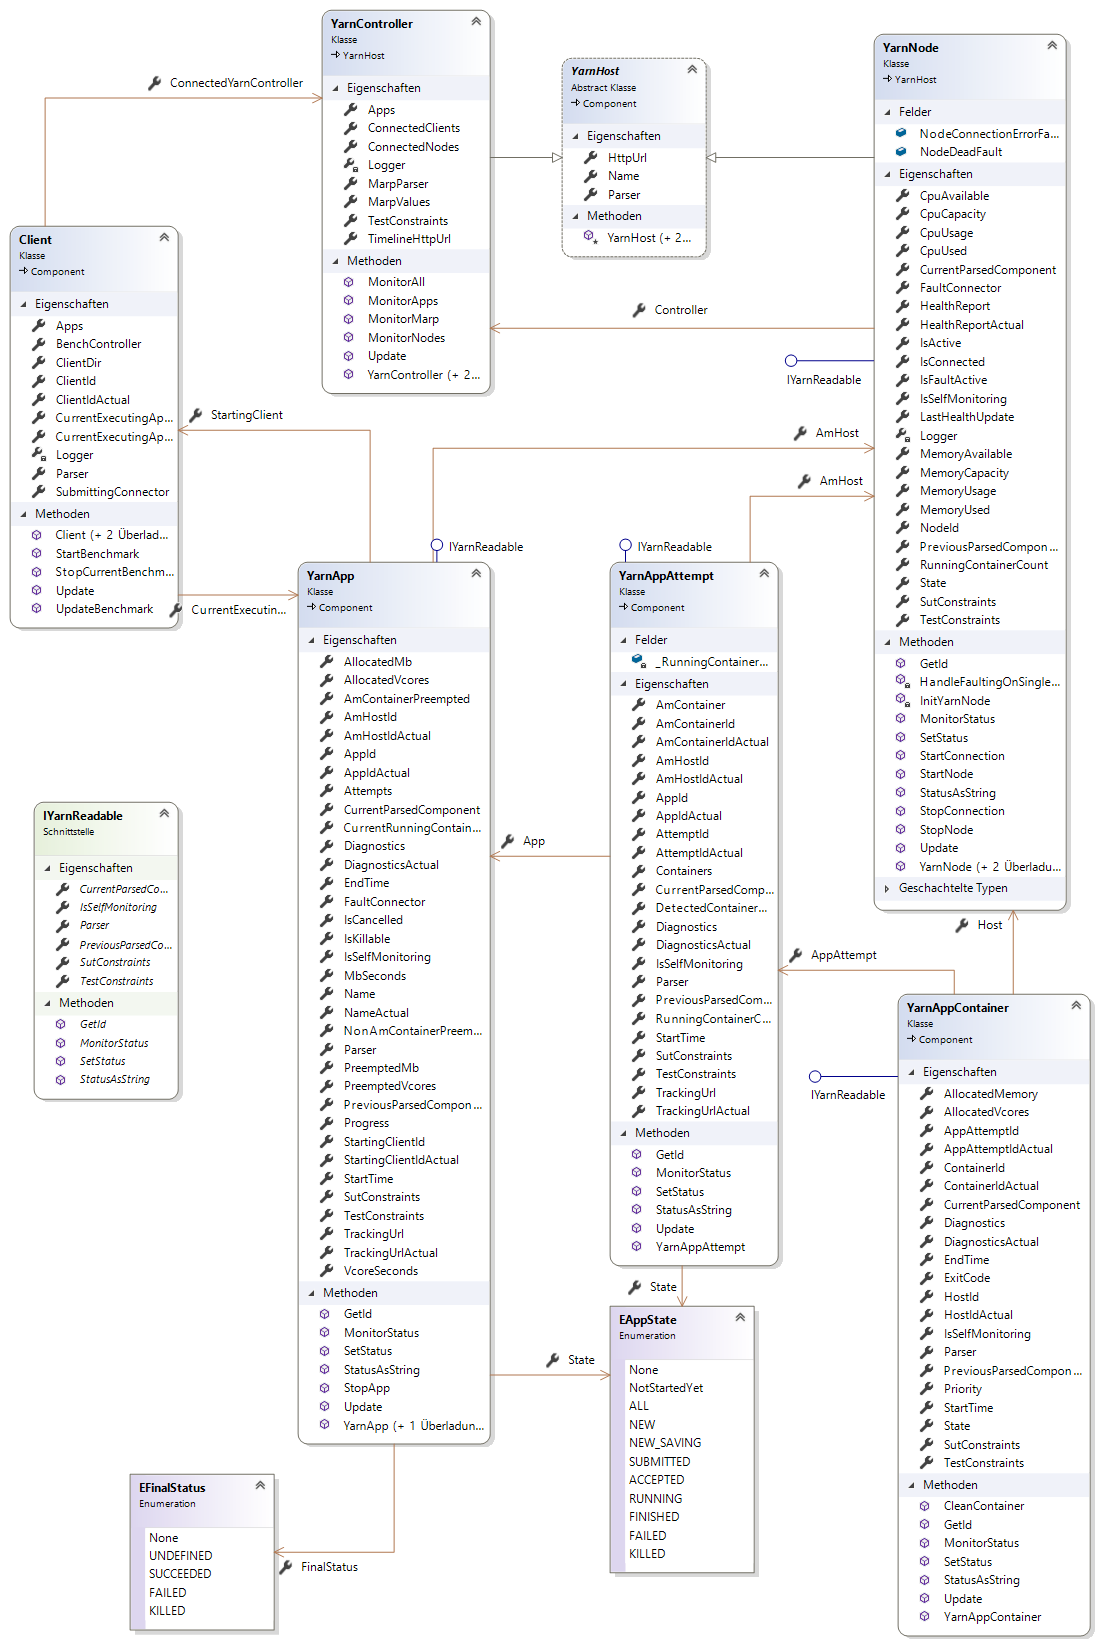
\includegraphics[width=\columnwidth]{./images/yarnModel.png}
	\caption[Aufbau des YARN-Modells]{Aufbau des YARN-Modells. Das Modell wurde mithilfe des Klassendiagramm-Designers in Visual Studio 2017 erstellt. Daher werden die aus Listen bestehenden Gegenassoziationen zu den Eigenschaften \texttt{YarnAppAttempt.App} (\texttt{YarnApp.Attempts}) und \texttt{YarnAppContainer.AppAttempt} (\texttt{YarnAppAttempt.Containers}) nicht im Diagramm angezeigt.}
	\label{fig:yarnModel}
\end{figure}

\autoref{fig:yarnModel} beschreibt im Grunde bereits das gesamte von \sS verwendete YARN-Modell. Enthalten sind alle hier relevanten Komponenten sowie deren Eigenschaften. Als Eigenschaften wurden jeweils alle Daten aufgenommen, welche mithilfe von Shell-Kommandos bzw. mithilfe der REST-API von YARN ermittelt werden kann.

Die abstrakte Basisklasse \texttt{YarnHost} stellt die Basis für alle Hosts des Clusters dar, also dem \texttt{YarnController} mit dem \ac{RM}, und dem \texttt{YarnNode}, was einen Node darstellt, auf dem die Anwendungen bzw. deren Container ausgeführt werden. Die abstrakte Eigenschaft \texttt{YarnHost.HttpPort} dient als Hilfs-Eigenschaft, da Controller und Nodes unterschiedliche Ports für die Weboberfläche nutzen, deren URL mit Port in der Eigenschaft \texttt{YarnHost.HttpUrl} abrufbar ist. Sie wird daher vom Controller bzw. Node mit dem entsprechenden Port versehen. Die Felder \texttt{YarnNode.NodeConnectionError} und \texttt{YarnNode.NodeDead} bilden die Komponentenfehler, wenn ein Node seine Netzwerkverbindung verliert bzw. beendet wird. Die Effekte der Komponentenfehler werden über entsprechende geschachtelte Typen bzw. innere Klassen realisiert.

Die Anwendungen, welche mit \texttt{YarnApp} dargestellt werden, werden mithilfe des \texttt{Client} gestartet, was den zu startenden Client darstellt. Die Anwendungen selbst enthalten neben grundlegenden Daten wie \zB den Namen auch einige Daten zum Ressourcenbedarf (Speicher und CPU). Zwar gibt Hadoop nicht direkt die zu der Anwendung gehörigen Job-Ausführungen an, allerdings können diese mithilfe der \texttt{YarnApp.AppId} sehr einfach ermittelt werden und dann in der Liste \texttt{YarnApp.Attempts} gespeichert werden. Das Feld \texttt{YarnApp.IsKillable} gibt an, ob die Ausführung der Anwendung mit den aktuellen Daten im Modell durch den Komponentenfehler \texttt{YarnApp.KillApp} abgebrochen werden kann. Abhängig ist das durch \texttt{YarnApp.FinalStatus}, was angibt, ob eine Anwendung erfolgreich ausgeführt wurde oder die Ausführung noch nicht abgeschlossen ist (durch \texttt{EFinalStatus.UNDEFINED}).

Jede Ausführung \texttt{YarnAppAttempt} hat eine eigene ID und Status und kann einer Anwendung zugeordnet werden. Genau wie bei den Anwendungen selber wird hier direkt der Node gespeichert, auf welchem der \ac{AppMstr} ausgeführt wird und einen eigenen Container bildet, dessen ID direkt gespeichert wird. Container (dargestellt durch \texttt{YarnAppContainer}) existieren in Hadoop nur während der Laufzeit eines Programmes und enthalten nur wenige Daten, darunter ihr ausführender Node. Jede Anwendung, deren Ausführungen und deren Container enthalten zudem den derzeitigen Status, ob die Komponente noch eingereicht wird, bereits ausgeführt wird oder beendet ist.

Alle vier YARN-Kernkomponenten implementieren das Interface \texttt{IYarnReadable}, was angibt, dass die Komponente ihren Status aus Hadoop ermitteln kann. Entsprechend wird in allen Komponenten die Methode \texttt{GetStatus()} implementiert, in welchem mithilfe des angegebenen Parsers auf den SSH-Treiber zugegriffen werden kann und die Komponenten im Modell so ihre Daten aus dem realen Cluster ermitteln können.
